\chapter{Casos de Uso} \label{cap:cap7}

Este capítulo apresenta alguns casos de uso onde as funcionalidades propostas nesta tese são pertinentes. 

\section{Multimodalidade} \label{sec:casoUsoMultimodalidade}

Esta seção apresenta casos de uso que explora deferentes modalidades de interação.

\subsection{Navegação multimodal}
A aplicação desenvolvida para ilustrar a combinação de modalidades diferentes de interação combina interação via voz e teclas do controle remoto. Ela possui três vídeos que poderão ser apresentados de acordo com o desejo do usuário. No primeiro momento, o usuário escolhe dentre três opções para exibir o primeiro vídeo. Selecionando um dos botões, o vídeo respectivo será apresentado. A interface inicial da aplicação é apresentada na Figura~\ref{fig:appMultmodal}. Após o início de qualquer um dos vídeos, o usuário poderá dizer ``trocar'' e então os botões com as opções aparecerão novamente possibilitando a troca do vídeo que está sendo apresentado. Ao selecionar outro vídeo, o atual será parado e o escolhido será exibido. A aplicação é apresentada na Listagem~\ref{lst:appIntMultModal}.

\begin{figure}[h!] 
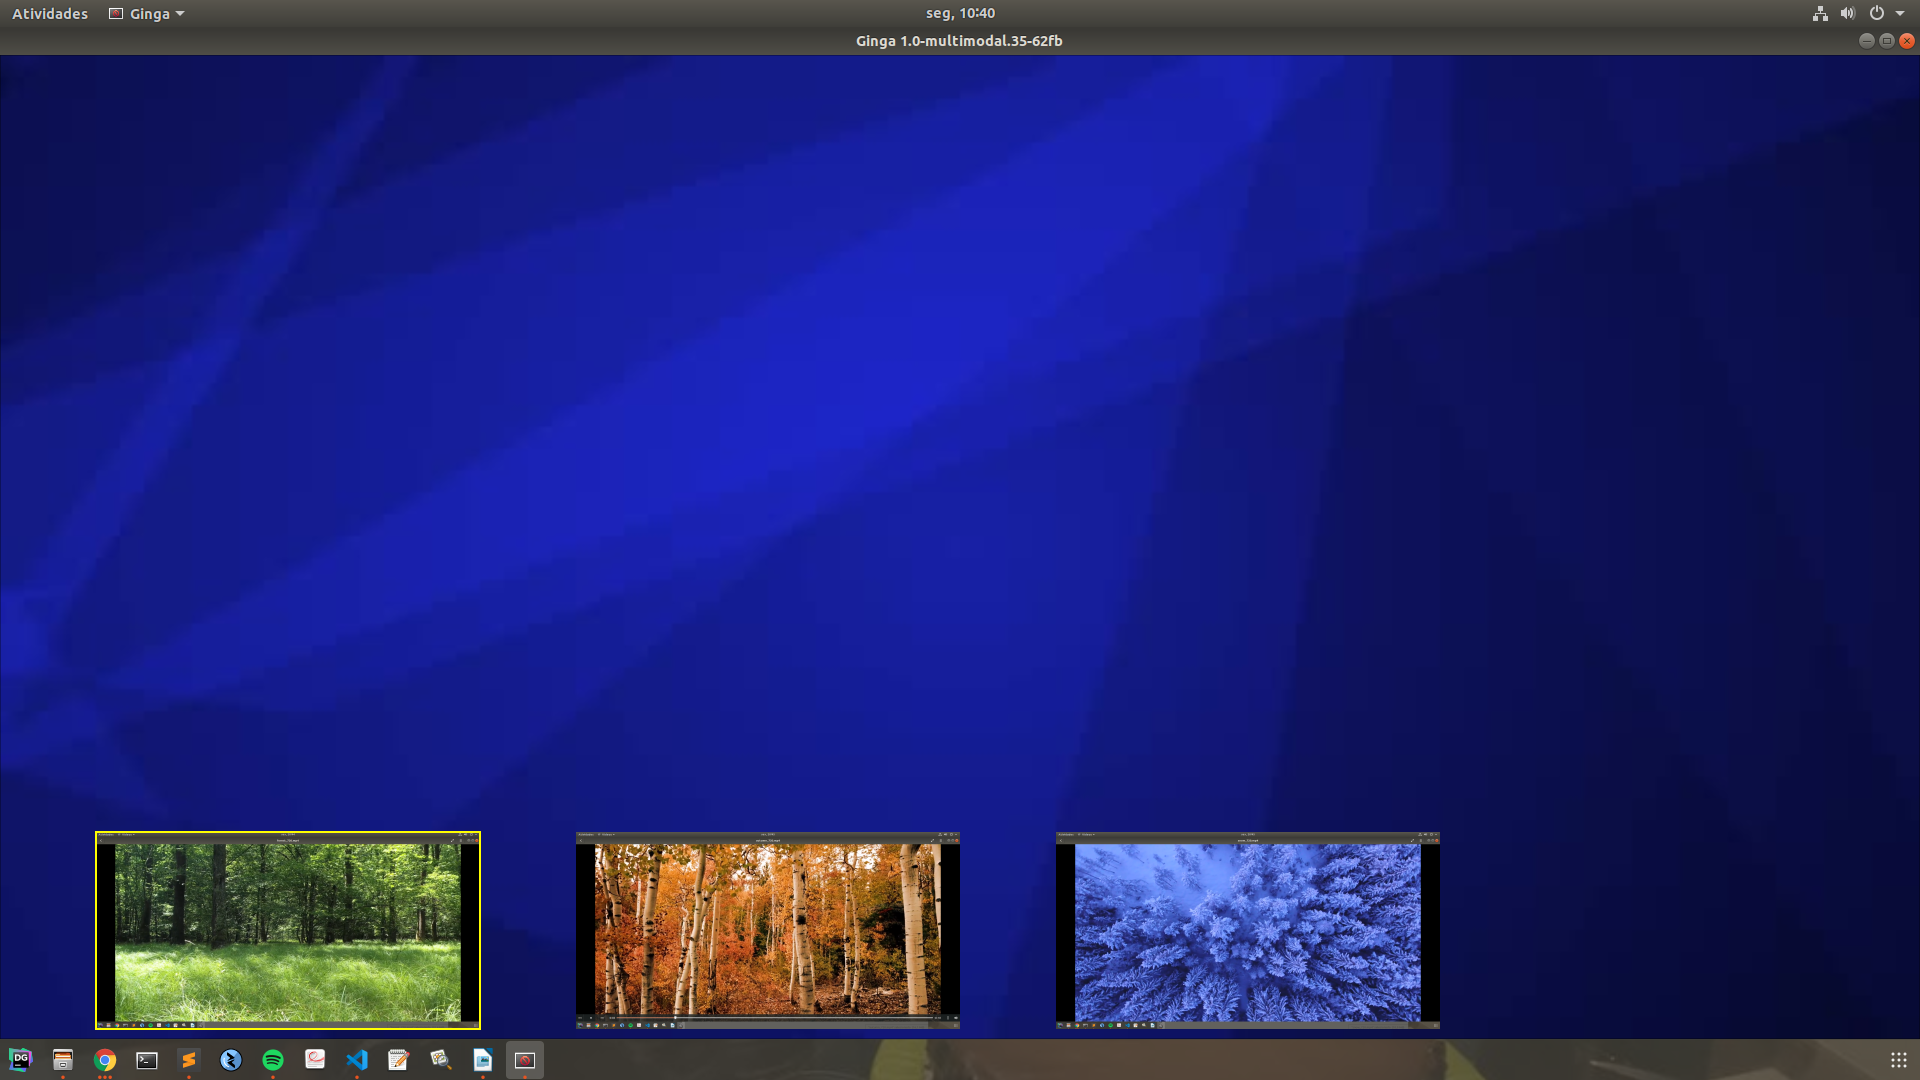
\includegraphics[scale=0.2]{figuras/appMultModal.png}
\centering
\caption{Interface da aplicação com interação multimodal na versão NCL 4.0.}
\label{fig:appMultmodal}
\end{figure}
\vspace{-0.2cm}

\begin{lstlisting}[language=ncl,label=lst:appIntMultModal, caption={Código da aplicação NCL com interação multimodal.}]
<?xml version="1.0" encoding="ISO-8859-1"?>
<ncl id="apNCL40MultModal" xmlns="http://www.ncl.org.br/NCL4.0/EDTVProfile">
 <head>
	<regionBase>
    <region id="backReg" width="100%" height="100%" zIndex="0" />
    <region id="florestaVideoReg" width="100%" height="100%" zIndex="1" />
    <region id="btnFlorestReg" bottom="5%" left="5%"  width="20%" height="20%" zIndex="2"/>
    <region id="btnAutumnReg" bottom="5%" left="30%" width="20%" height="20%" zIndex="2"/>
    <region id="btnSnowReg"    bottom="5%" left="55%" width="20%" height="20%" zIndex="2"/>
	</regionBase>

	<descriptorBase>
      <descriptor id="backDesc"  region="backReg"/>
      <descriptor id="florestaVideoRegDesc"  region="florestaVideoReg"/>
      <descriptor id="btnFlorestDesc" region="btnFlorestReg" focusIndex="0" moveUp="2" moveDown="1" moveLeft="2" moveRight="1" focusBorderColor="yellow" focusBorderWidth="2"/>
      <descriptor id="btnAutumnDesc" region="btnAutumnReg" focusIndex="1" moveUp="0" moveDown="2" moveLeft="0" moveRight="2" focusBorderColor="yellow" focusBorderWidth="2"/>
      <descriptor id="btnSnowDesc" region="btnSnowReg"    focusIndex="2" moveUp="1" moveDown="0" moveLeft="1" moveRight="0" focusBorderColor="yellow" focusBorderWidth="2" />
	</descriptorBase>
	<connectorBase>
       <causalConnector id="onVoiceRecognitionStart">
          <connectorParam name="key"/>
          <connectorParam name="user"/>      
          <simpleCondition role="onVoiceRecognition" key="$\$$key" user="$\$$user"/>
          <simpleAction role="start" max="unbounded"/>
       </causalConnector>  
       <causalConnector id="onBeginStart">
          <simpleCondition role="onBegin"/>
          <simpleAction role="start" max="unbounded"/>
       </causalConnector>  
       <causalConnector id="onSelectionStartStop">
          <simpleCondition role="onSelection"/>
          <compoundAction operator="seq">
              <simpleAction role="start" max="unbounded"/>
              <simpleAction role="stop" max="unbounded"/>
          </compoundAction>
       </causalConnector>  
       <causalConnector id="onBeginStop">
          <simpleCondition role="onBegin"/>
          <simpleAction role="stop" max="unbounded"/>
       </causalConnector>  
	 </connectorBase>
</head>
<body>
	<port id="pBack" component="back" />
    <media id="back" src="images/blue.jpg" descriptor="backDesc"/>
    <media id="florestVideo" src="videos/forest_720.mp4" descriptor="florestaVideoRegDesc"/>
    <media id="autumnVideo" src="videos/autumn_720.mp4" descriptor="florestaVideoRegDesc"/>
    <media id="snowVideo" src="videos/snow_720.mp4" descriptor="florestaVideoRegDesc"/>
    <media id="btnFlorestVideo" src="images/florest.png" descriptor="btnFlorestDesc"/>
    <media id="btnAutumnVideo" src="images/autumn.png" descriptor="btnAutumnDesc"/>
    <media id="btnSnowVideo" src="images/snow.png" descriptor="btnSnowDesc"/>
    <link xconnector="onBeginStart">
          <bind role="onBegin" component="back"/>
          <bind role="start" component="btnFlorestVideo"/>
          <bind role="start" component="btnAutumnVideo"/>
          <bind role="start" component="btnSnowVideo"/>
    </link> 
    <link xconnector="onBeginStop">
          <bind role="onBegin" component="florestVideo"/>
          <bind role="stop" component="btnFlorestVideo"/>
          <bind role="stop" component="btnAutumnVideo"/>
          <bind role="stop" component="btnSnowVideo"/>
    </link> 
   <link xconnector="onBeginStop">
          <bind role="onBegin" component="autumnVideo"/>
          <bind role="stop" component="btnFlorestVideo"/>
          <bind role="stop" component="btnAutumnVideo"/>
          <bind role="stop" component="btnSnowVideo"/>
    </link> 
   <link xconnector="onBeginStop">
          <bind role="onBegin" component="snowVideo"/>
          <bind role="stop" component="btnFlorestVideo"/>
          <bind role="stop" component="btnAutumnVideo"/>
          <bind role="stop" component="btnSnowVideo"/>
    </link> 
    <link xconnector="onSelectionStartStop">
      <bind role="onSelection" component="btnSnowVideo"/>
      <bind role="start" component="snowVideo"/>
      <bind role="stop" component="autumnVideo"/>
      <bind role="stop" component="florestVideo"/>
    </link> 
    <link xconnector="onSelectionStartStop">
      <bind role="onSelection" component="btnFlorestVideo"/>
      <bind role="start" component="florestVideo"/>
      <bind role="stop" component="autumnVideo"/>
      <bind role="stop" component="snowVideo"/>
    </link> 
    <link xconnector="onSelectionStartStop">
      <bind role="onSelection" component="btnAutumnVideo"/>
      <bind role="start" component="autumnVideo"/>
      <bind role="stop" component="snowVideo"/>
      <bind role="stop" component="florestVideo"/>
    </link>  
    <link xconnector="onVoiceRecognitionStart">
          <bind role="onVoiceRecognition" component="back">
            <bindParam name="key" value="trocar"/>
          </bind>
          <bind role="start" component="btnFlorestVideo"/>
          <bind role="start" component="btnAutumnVideo"/>
          <bind role="start" component="btnSnowVideo"/>
    </link> 
 </body>
</ncl>
\end{lstlisting}

\subsection{Caso "\textit{Put That There}"}

Turk et al.\cite{turk2014multimodal} discute sobre como o famoso "\textit{Put That There}" de Bolt et. al.\cite{bolt1980put} abriu caminho para vários sistemas que pretendem integrar diferentes modos de interação em uma variedade de áreas de aplicação. Os primeiros sistemas multimodais focavam principalmente em tarefas espaciais e aplicativos baseados em mapas. Em \cite{bolt1980put}, os comandos de voz "\textit{Put that}" e "\textit{there}" processados em conjunto com o gesto de apontar destacam a grande utilidade da interação multimodal em um sistema de gerenciamento de dados espaciais. Assim, como prova de conceito e para ilustrar um caso de uso pertinente para os usuários de DTV, esta seção apresenta uma aplicação que usa esse exemplo de interação multimodal no contexto de uma experiência de DTV. Com a diferença que na aplicação, o usuário seleciona com o controle remoto.

A aplicação representa um cenário onde o usuário assiste a uma partida de futebol apresentada na TV e dois objetos de mídia sobrepostos ao vídeo principal: o placar e o vídeo do narrador, como podemos ver na Figura~\ref{fig:putThat1}. O usuário selecionar o placar ou o vídeo do narrador e mudar sua posição na tela. Assim que o usuário selecionar um objeto de mídia e disser "\textit{put that}", ele será "pego". Em seguida, as novas regiões espaciais para possíveis deslocamentos aparecem na TV. O usuário então seleciona a região para a qual deseja que a mídia seja movida e diz "\textit{there}".

A Figura~\ref{fig:putThat2} mostra como a aplicação apresenta duas novas regiões superiores possíveis no momento exato em que o usuário seleciona o placar e diz "\textit{put that}". A Figura~\ref{fig:putThat3} mostra o ponto esquerdo escolhido logo após o usuário ter selecionado. Quando ele diz "there", o aplicativo altera o placar colocando-o no local selecionado, conforme mostrado na Figura~\ref{fig:putThat4}. Depois disso, os pontos de movimento desaparecem, como podemos ver na Figura~\ref{fig:putThat5}.

\begin{figure}
  \subfloat[Estado inicial]
  {
    \label{fig:putThat1}
	\begin{minipage}[c][1\width]{0.48\textwidth}
	   \centering
	   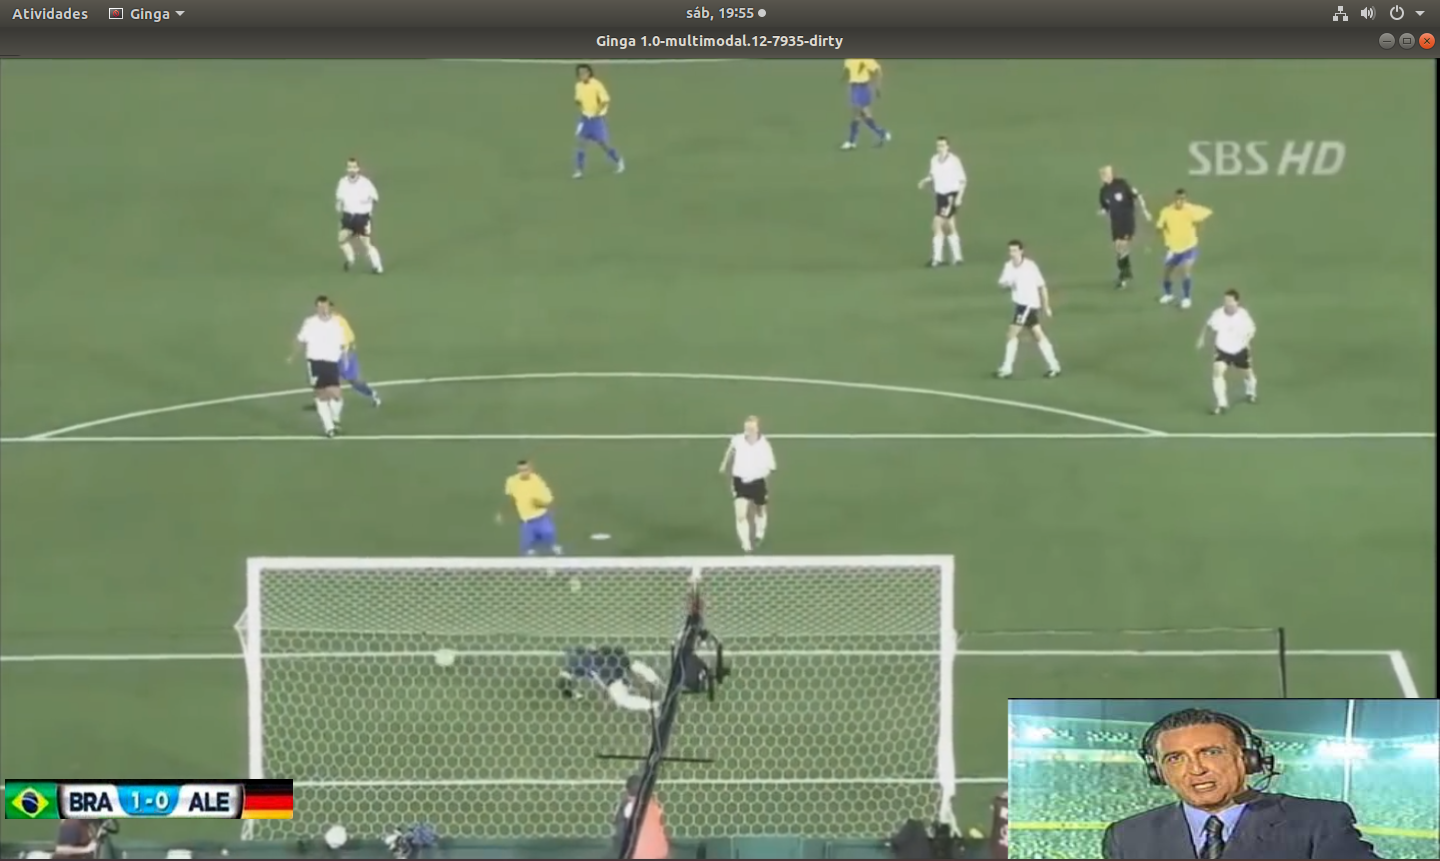
\includegraphics[width=1\textwidth]{figuras/Jogo1.png}
	   \vspace{-2.5cm}
	\end{minipage}
  } \hfill 	
  \subfloat[Depois que o usuário disser "put that"]
  {
    \label{fig:putThat2}
	\begin{minipage}[c][1\width]{0.48\textwidth}
	   \centering
	   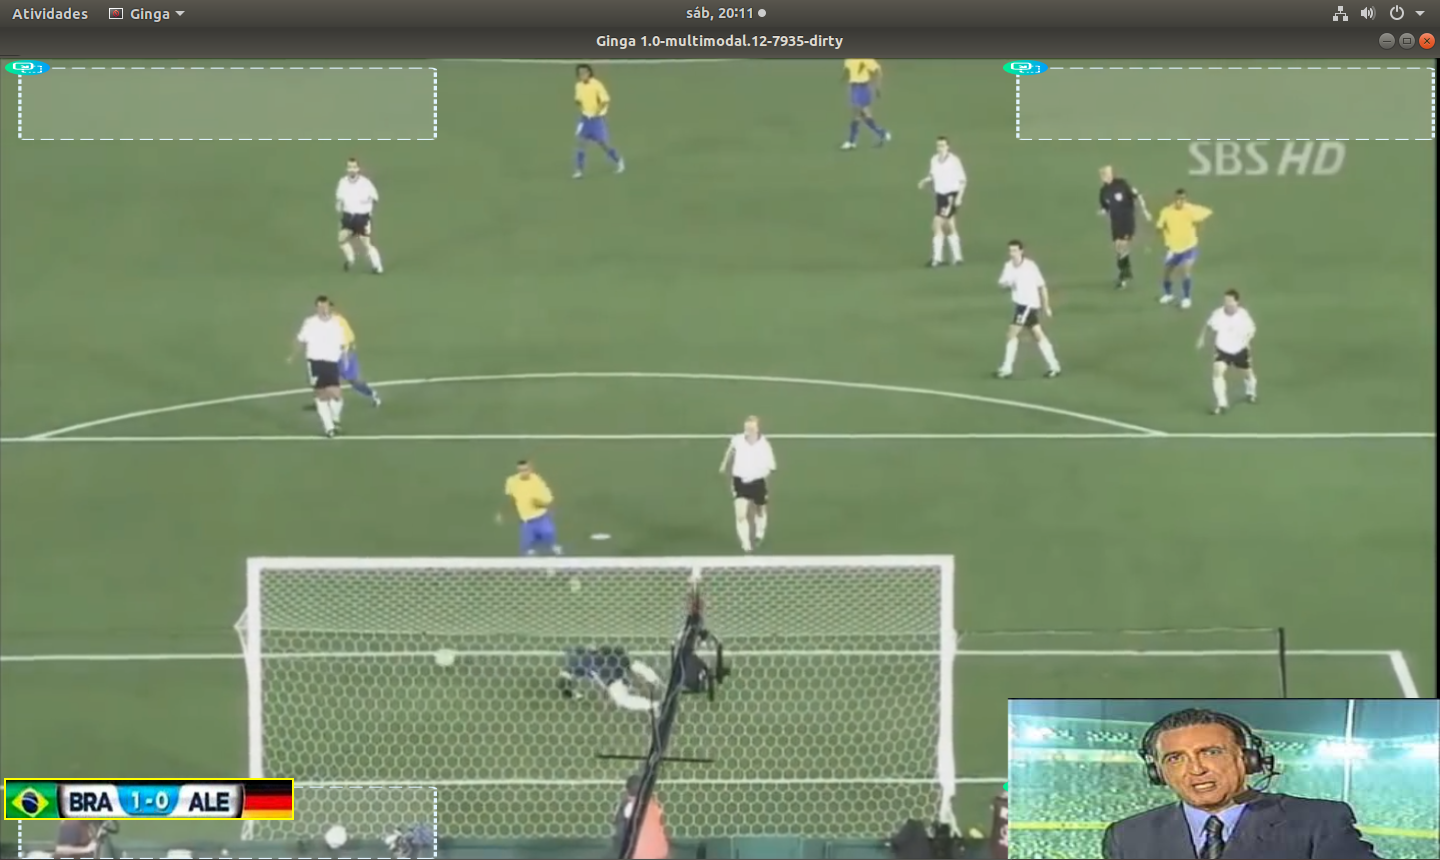
\includegraphics[width=1\textwidth]{figuras/Jogo2.png}
	   \vspace{-2.5cm}
	\end{minipage}
  }
  \vspace{-2cm}
  \newpage
  \subfloat[Depois que o usuário seleciona o ponto esquerdo]
  {
    \label{fig:putThat3}
	\begin{minipage}[c][1\width]{0.48\textwidth}
	   \centering
	   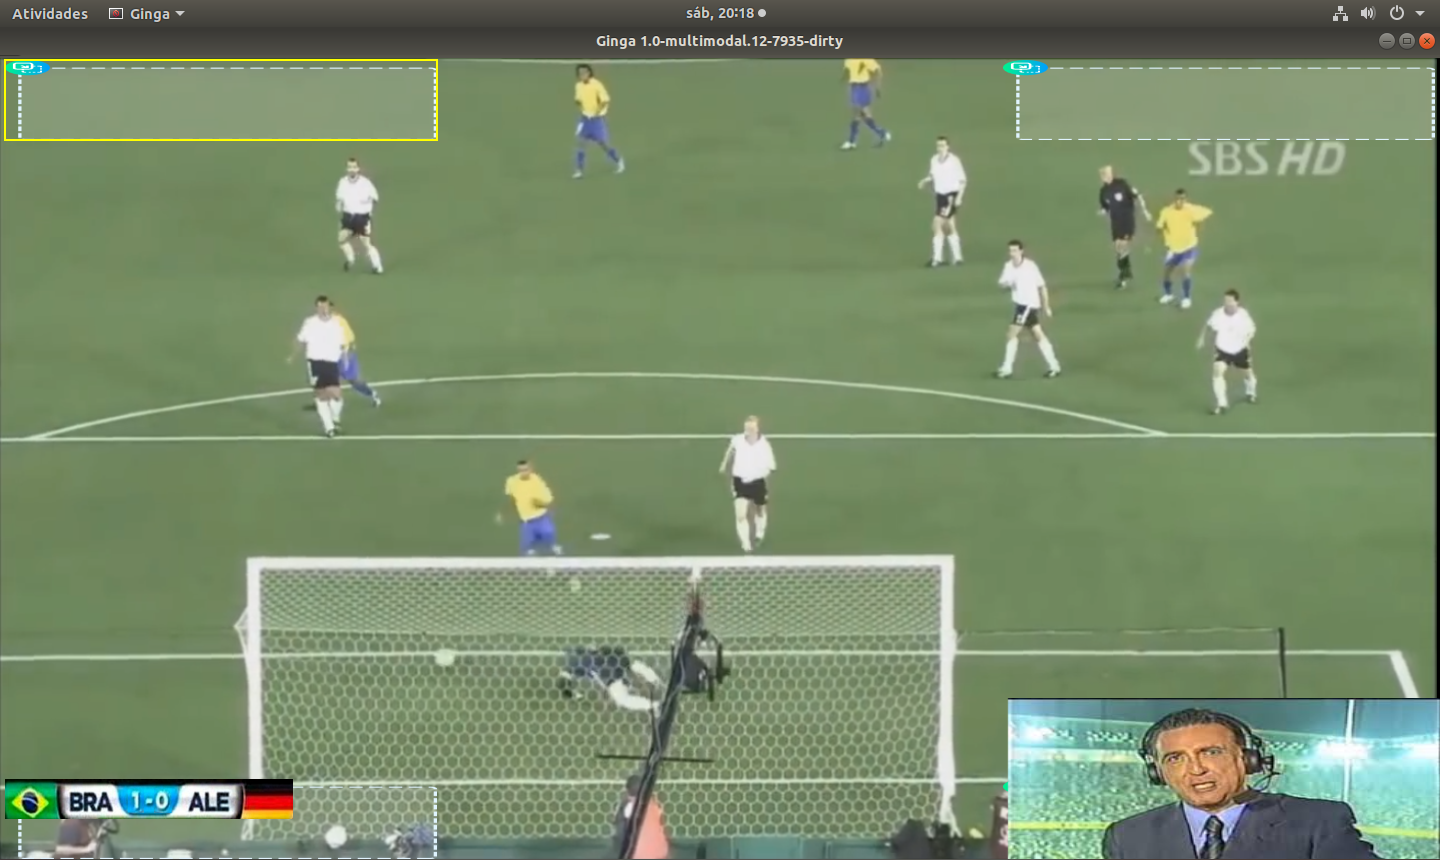
\includegraphics[width=1\textwidth]{figuras/Jogo3.png}
	   \vspace{-2.5cm}
	\end{minipage}
   } \hfill 	
   \subfloat[Depois que o usuários disser "there"]
   {
	\label{fig:putThat4}
	\begin{minipage}[c][1\width]{0.48\textwidth}
	   \centering
	   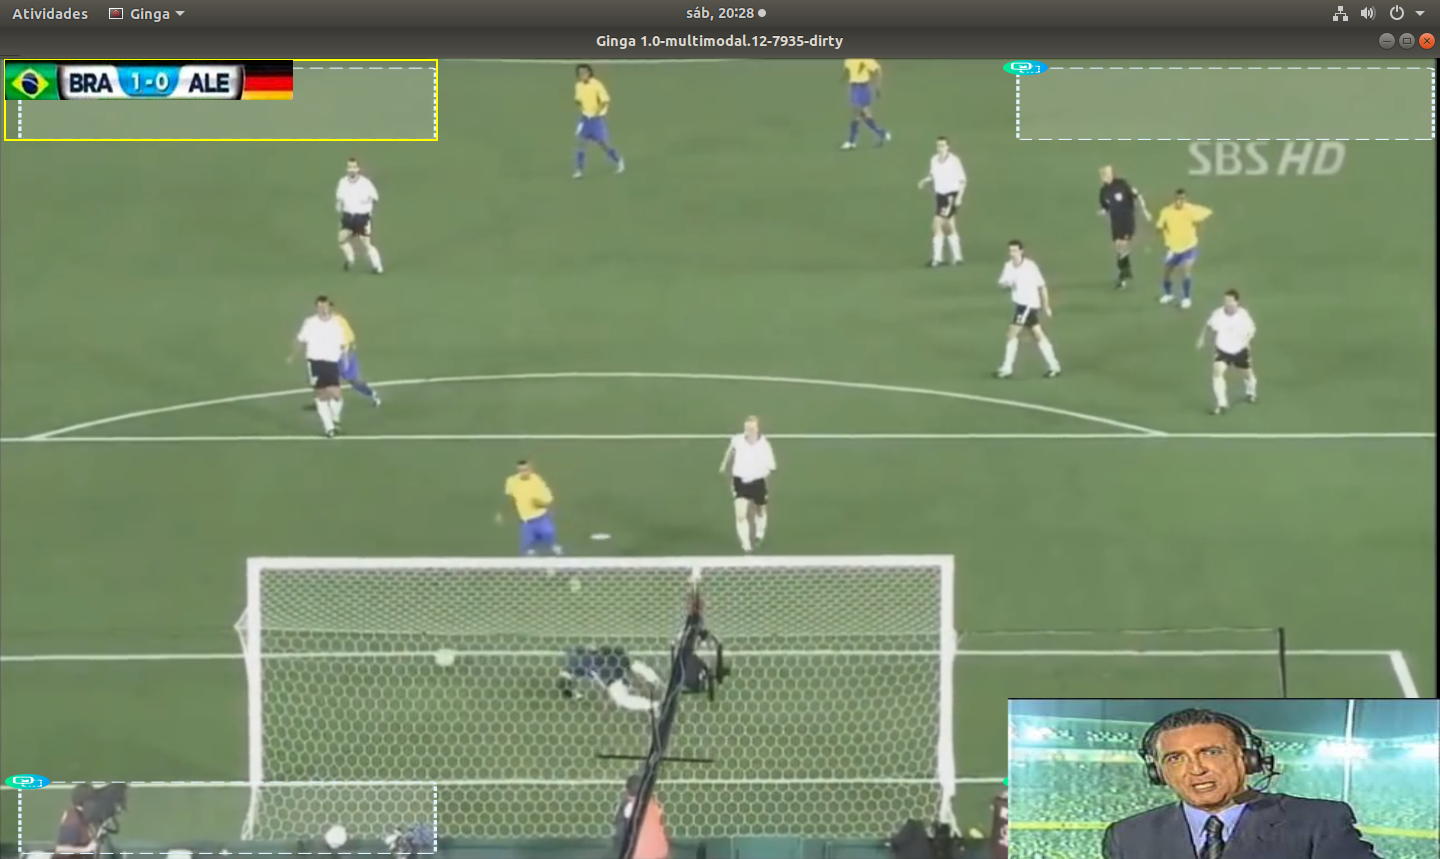
\includegraphics[width=1\textwidth]{figuras/Jogo4.png}
	   \vspace{-2.5cm}
	\end{minipage}
   }
	\vspace{-2cm}
	\newpage
	\begin{center}
	\subfloat[Depois que a interação terminar]
	{
	  \label{fig:putThat5}
	  \begin{minipage}[c][1\width]{
	   0.6\textwidth}
	   \centering
	   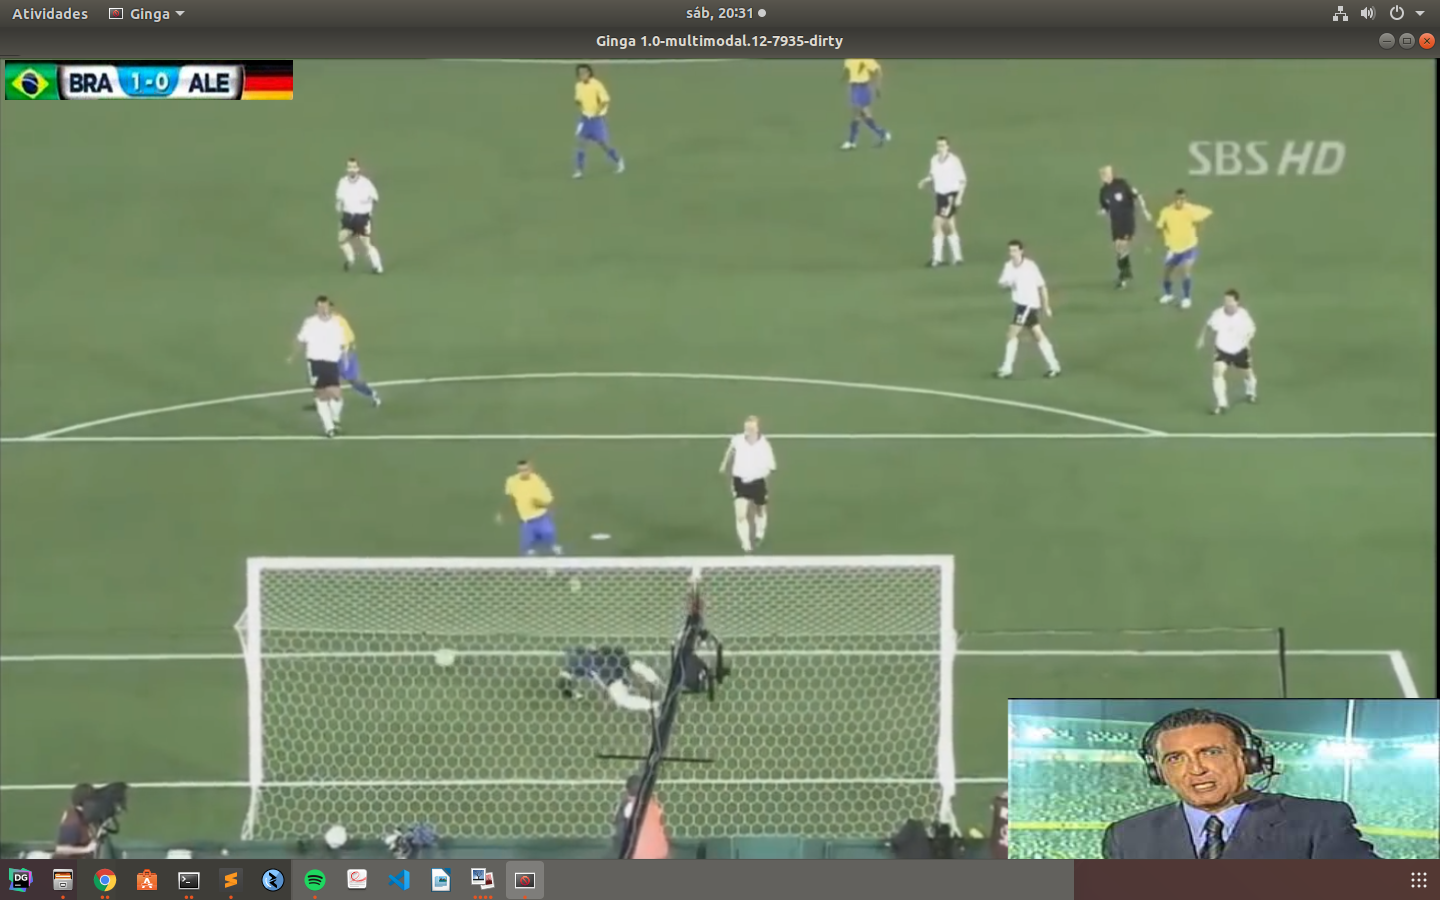
\includegraphics[width=1\textwidth]{figuras/Jogo5.png}
	   \vspace{-2.5cm}
	  \end{minipage}
	}
	\end{center}
\caption{Instantes do aplicativo em execução após cada interação do usuário}
\end{figure}


\section{Multiusuário} \label{sec:casoUsoMultiusuario}

Nesta seção apresenta casos de uso onde a participação e identificação do usuário representa uma interessante funcionalidade tendo em vista a importância da participação da TV Digital na vida das pessoas.  

\subsection{Limitação de interação} \label{sec:casoUsoLimiteInteracao}
Neste caso de uso, somente os usuários \textit{U01} e \textit{U02} atendem o perfil. Suas propriedades, incluindo o \textit{id}, estão armazenadas nos arquivos \textit{usr1.xml} e \textit{usr2.xml} respectivamente. A aplicação é apresentada na Listagem~\ref{lst:appIdMultUser}.

\begin{lstlisting}[language=ncl,label=lst:appIdMultUser, caption={Código da aplicação NCL com identificação multiusuário.}]
<?xml version="1.0" encoding="ISO-8859-1"?>
<ncl id="aplNCL40MultUser" xmlns="http://www.ncl.org.br/NCL4.0/EDTVProfile">
 <head>
	<regionBase>
		<region id="florestaVideoReg" width="100%" height="100%" zIndex="0" />
	</regionBase>
	<descriptorBase>
	    <descriptor id="florestaVideoRegDesc"  region="florestaVideoReg" />
	</descriptorBase>
	<connectorBase>
       <causalConnector id="onVoiceRecognitionPause">
          <connectorParam name="key"/>
          <connectorParam name="user"/>      
          <simpleCondition role="onVoiceRecognition" key="$\$$key" user="$\$$user"/>
          <simpleAction role="pause" />
       </causalConnector>  
       <causalConnector id="onVoiceRecognitionResume">
          <connectorParam name="key"/>
          <connectorParam name="user"/>      
          <simpleCondition role="onVoiceRecognition" key="$\$$key" user="$\$$user"/>
          <simpleAction role="resume" />
       </causalConnector>  
       <causalConnector id="onVoiceRecognitionStop">
          <connectorParam name="key"/>
          <connectorParam name="user"/>      
          <simpleCondition role="onVoiceRecognition" key="$\$$key" user="$\$$user"/>
          <simpleAction role="stop" />
       </causalConnector>  
	</connectorBase>
    <userBase>
      <userProfile id="profile1" src="profiles/profile.xml"/>
    </userBase>
  </head>
<body>
	<port id="pVideo" component="florestaVideo" />
	<media id="florestaVideo" src="videos/forest_720.mp4" descriptor="florestaVideoRegDesc"/>
    <link xconnector="onVoiceRecognitionPause">
          <bind role="onVoiceRecognition" component="florestaVideo">
            <bindParam name="key" value="pausar"/>
            <bindParam name="user" value="profile1"/>
          </bind>
          <bind role="pause" component="florestaVideo"/>
    </link> 
    <link xconnector="onVoiceRecognitionResume">
          <bind role="onVoiceRecognition" component="florestaVideo">
            <bindParam name="key" value="tocar"/>
            <bindParam name="user" value="profile1"/>            
          </bind>
          <bind role="resume" component="florestaVideo"/>
    </link> 
    <link xconnector="onVoiceRecognitionStop">
          <bind role="onVoiceRecognition" component="florestaVideo">
            <bindParam name="key" value="parar"/>
            <bindParam name="user" value="profile1"/>            
          </bind>
          <bind role="stop" component="florestaVideo"/>
    </link> 
 </body>
</ncl>
\end{lstlisting}

\subsection{Identificação do usuário} \label{sec:casoUsoIdentificaçãoInteracao}

A aplicação desenvolvida possui uma mídia que será executada com o início do documento NCL. O conteúdo do vídeo apresenta uma floresta com neve e em um determinado momento será apresentada uma imagem vendendo um passeio de esqui. No momento que o usuário diz ``comprar'', a aplicação vai informar quem comprou o passeio identificando a interação. Porém, aplicação só irá responder se a interação vier de um dos usuários que atendem o perfil definido no profile. A aplicação é apresentada na Listagem~\ref{lst:appIntMultUser}.

\begin{figure}[h!] 
    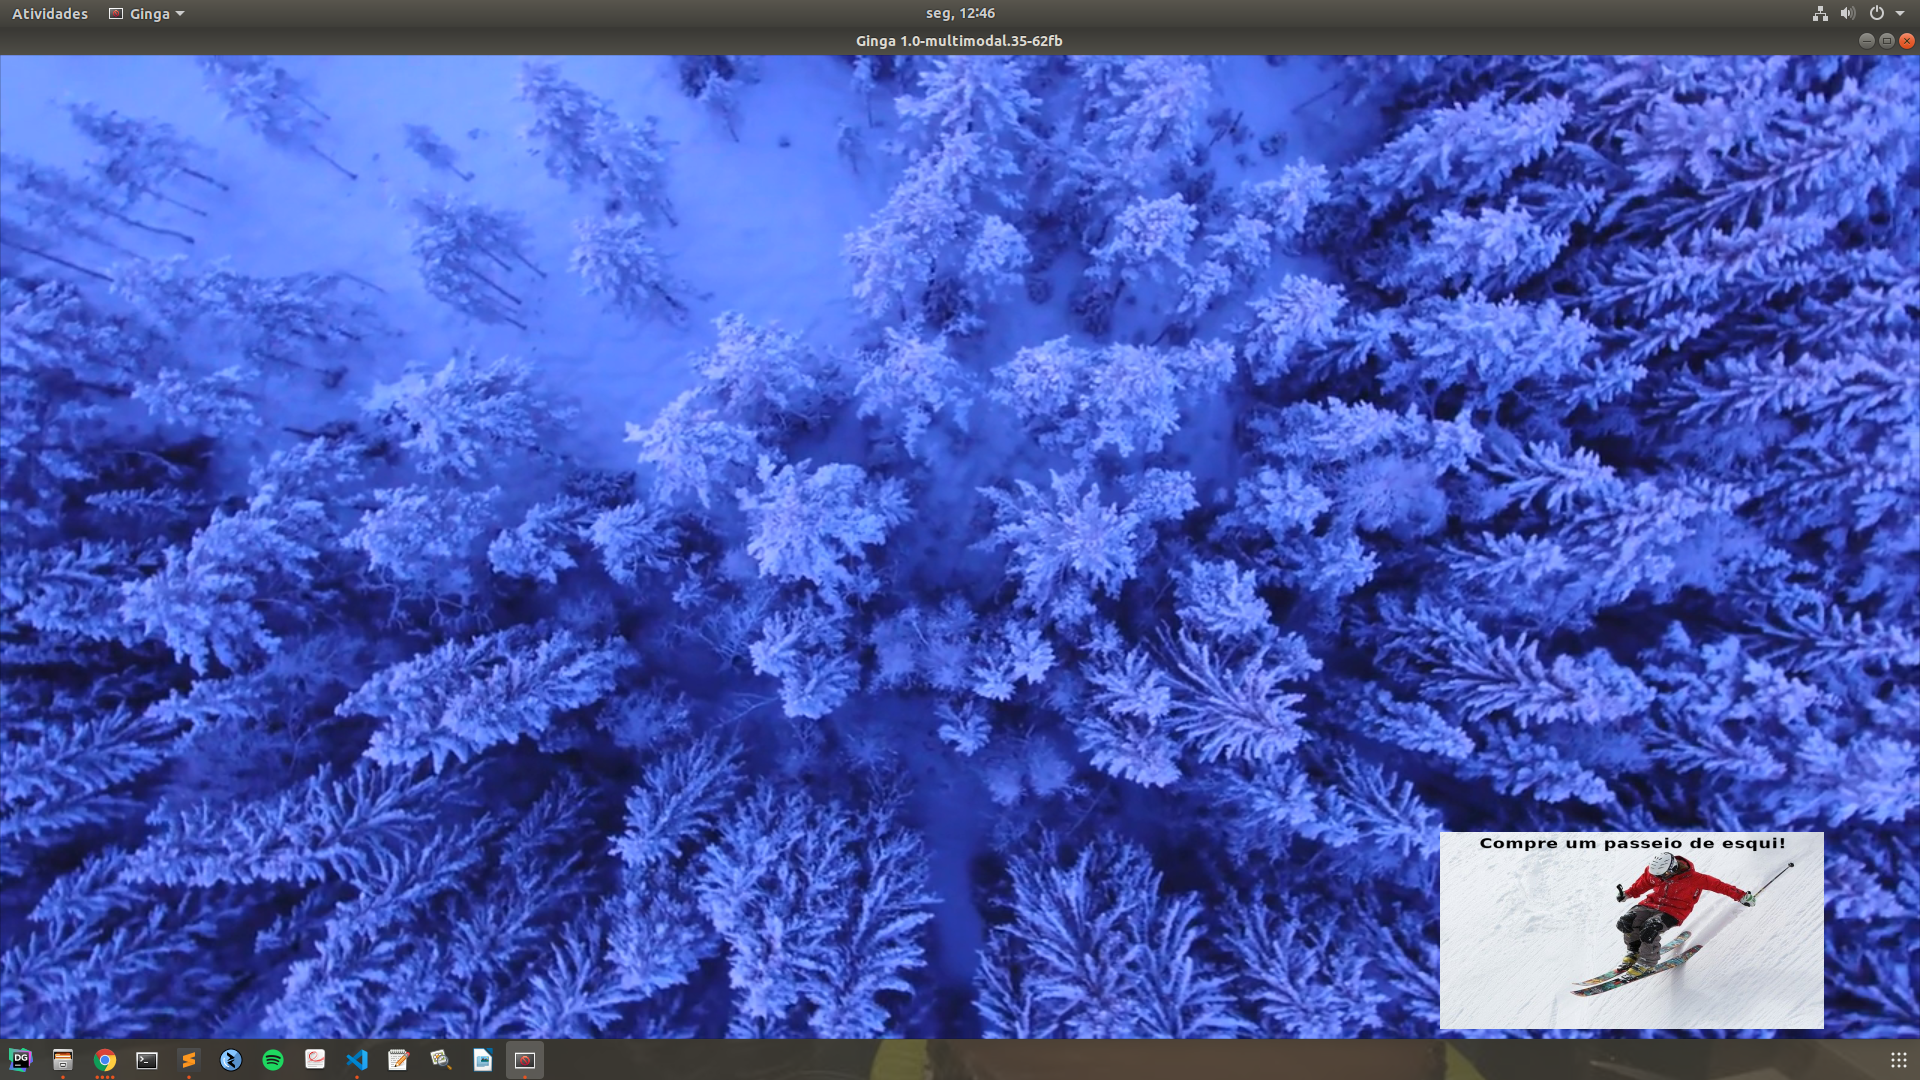
\includegraphics[scale=0.2]{figuras/appMultUser.png}
    \centering
    \caption{Interface da aplicação com interação multiuser.}
    \label{fig:appMultUser}
\end{figure}
\vspace{-0.2cm}

\begin{lstlisting}[language=ncl,label=lst:appIntMultUser, caption={Código da aplicação NCL com interação multiusuário.}]
<?xml version="1.0" encoding="ISO-8859-1"?>
<ncl id="aplMultiUser" xmlns="http://www.ncl.org.br/NCL3.0/EDTVProfile">
<head>
  <regionBase>
    <region id="VideoReg" width="100%" height="100%" zIndex="0" />
    <region id="ImgPropagandaReg" right="5%" bottom="5%" width="20%" height="20%" zIndex="2"/>  
    <region id="rg1" left="5%" bottom="5%" height="10%"  width="50%" />
  </regionBase>
  <descriptorBase>
      <descriptor id="VideoDesc"  region="VideoReg"/>  
      <descriptor id="ImgPropagandaDesc"  region="ImgPropagandaReg"  />
      <descriptor id="desc1"  region="rg1"/> 
  </descriptorBase>
  <userBase>
      <userProfile id="profile1" src="profiles/profile.xml"/>
  </userBase>
  <connectorBase>
      <causalConnector id="onBeginStart">
        <simpleCondition role="onBegin"/>
        <simpleAction role="start" max="unbounded"/>
      </causalConnector> 
      <causalConnector id="onVoiceRecognitionSet">
        <connectorParam name="key"/>
        <connectorParam name="user"/>      
        <connectorParam name="var"/>      
        <simpleCondition role="onVoiceRecognition" key="$\$$key" user="$\$$user"/>
        <simpleAction role="set" value="$\$$var"/>
      </causalConnector>
  </connectorBase>
</head>
<body>
    <port id="pInicio" component="lua" />
    <port id="pVideo" component="snowVideo"/>
    <media id="lua" src="scripts/script.lua" type= "application/x-ginga-NCLua" descriptor="desc1">
      <property name="usr" value="false"/>
    </media>
    <media id="ImgPropaganda" src="images/passeioEsqui.jpeg" descriptor="ImgPropagandaDesc">
      <property name="usr" value="false"/>
    </media>
    <media id="snowVideo" src="videos/snow_720.mp4" descriptor="VideoDesc">
      <property name="usr" value="false"/>
      <area id="aPropaganda" begin="2s" /> 
    </media>
    <link xconnector="onBeginStart">
        <bind role="onBegin" component="snowVideo" interface="aPropaganda"/>
        <bind role="start" component="ImgPropaganda"/>
    </link>
    <link xconnector="onVoiceRecognitionSet">
      <bind role="onVoiceRecognition" component="ImgPropaganda">
          <bindParam name="key" value="comprar"/>
          <bindParam name="user" value="profile1"/>
      </bind> 
      <bind role="getValue" component="ImgPropaganda" interface="usr"/>
        <bind role="set" component="lua" interface="usr">
            <bindParam name="var" value="$\$$getValue"/>
        </bind>
    </link>
</body>
</ncl>
\end{lstlisting}

No próximo capitulo será abordado as considerações finais desta tese contendo conclusões e trabalhos futuros.


